% =============================================================================
% Lecture 3: Climate Change and Common Resources
% =============================================================================
\documentclass[9pt,english,aspectratio=169]{beamer}
% =============================================================================
% Pathways: Economics & Finance Workshop — Beamer Preamble
% =============================================================================
% Usage: Each lecture .tex file should start with:
%   \documentclass[10pt,english,aspectratio=169]{beamer}
%   % =============================================================================
% Pathways: Economics & Finance Workshop — Beamer Preamble
% =============================================================================
% Usage: Each lecture .tex file should start with:
%   \documentclass[10pt,english,aspectratio=169]{beamer}
%   % =============================================================================
% Pathways: Economics & Finance Workshop — Beamer Preamble
% =============================================================================
% Usage: Each lecture .tex file should start with:
%   \documentclass[10pt,english,aspectratio=169]{beamer}
%   \input{../../codes/Preambles/header_slides}
% Compile: cd output/Slides && TEXINPUTS=../../codes/Preambles:$TEXINPUTS xelatex file.tex
% =============================================================================

% ---------- Packages ----------
% Fonts
\usepackage{lmodern}
\usepackage[utf8]{inputenc}
\usepackage[normalem]{ulem}

% Math
\usepackage{amsmath,amssymb,amsthm}

% Figures and tables
\usepackage{graphicx}
\usepackage{array,tabularx,booktabs,threeparttable}

% TikZ and pgfplots
\usepackage{pgfplots}
\pgfplotsset{compat=1.18}
\usepackage{tikz}
\usetikzlibrary{positioning,arrows.meta,calc}

% Colored boxes
\usepackage[most]{tcolorbox}

% Miscellaneous
\usepackage{transparent}
\usepackage{setspace}
\usepackage[nodayofweek]{datetime}
\usepackage{hyperref}

% ---------- Theme ----------
\usetheme{CambridgeUS}
\usecolortheme{dolphin}
\usepackage{appendixnumberbeamer}

% ---------- Itemize ----------
\setbeamercovered{invisible}
\setbeamertemplate{itemize items}[default]
\setbeamertemplate{enumerate items}[default]

\setbeamertemplate{itemize item}[triangle]
\setbeamertemplate{itemize subitem}[triangle]
\setbeamertemplate{itemize subsubitem}{-}

% ---------- Headline / Footline ----------
\setbeamertemplate{headline}{}

\setbeamertemplate{footline}{
  \leavevmode
  \hbox{
    \begin{beamercolorbox}[wd=\paperwidth,ht=2.5ex,dp=1.25ex,leftskip=1em,rightskip=1em]{footline}
      \hfill \insertframenumber
    \end{beamercolorbox}
  }
}

\setbeamertemplate{navigation symbols}{}

% ---------- Frame title (centered) ----------
\makeatletter
\setbeamertemplate{frametitle}{
  \nointerlineskip
  \begin{beamercolorbox}[wd=\paperwidth,sep=0.35cm,center]{frametitle}
    {\usebeamerfont{frametitle}\insertframetitle\par}
    \ifx\insertframesubtitle\@empty\else
      \vspace{0.15cm}
      {\usebeamerfont{framesubtitle}\usebeamercolor[fg]{framesubtitle}\insertframesubtitle\par}
    \fi
  \end{beamercolorbox}
}
\makeatother

% ---------- Margins ----------
\setbeamersize{
  text margin left=2em,
  text margin right=2em
}

% ---------- Section outline frames ----------
\AtBeginSection[]{
  \begin{frame}{Outline}
    \tableofcontents[currentsection,
                     currentsubsection,
                     hideothersubsections]
  \end{frame}
}

% =============================================================================
% Colors — Okabe-Ito colorblind-friendly palette
% =============================================================================

\definecolor{black}{HTML}{000000}
\definecolor{orange}{HTML}{E69F00}
\definecolor{skyblue}{HTML}{56B4E9}
\definecolor{green}{HTML}{009E73}
\definecolor{yellow}{HTML}{F0E442}
\definecolor{blue}{HTML}{0072B2}
\definecolor{vermillion}{HTML}{D55E00}
\definecolor{purple}{HTML}{CC79A7}

% Semantic aliases (mapped to Okabe-Ito)
\definecolor{softbg}{HTML}{F5F5F5}
\definecolor{lightgray}{gray}{0.65}

% =============================================================================
% Box Environments
% =============================================================================

% --- Key points (orange background) ---
\newtcolorbox{keybox}{
  colback=orange!12,
  colframe=orange,
  fonttitle=\bfseries,
  boxrule=0.5pt,
  arc=2pt,
  left=6pt,
  right=6pt,
  top=4pt,
  bottom=4pt
}

% --- Highlights (orange left accent) ---
\newtcolorbox{highlightbox}{
  colback=white,
  colframe=orange,
  fonttitle=\bfseries,
  boxrule=0pt,
  leftrule=3pt,
  arc=0pt,
  left=6pt,
  right=6pt,
  top=4pt,
  bottom=4pt
}

% --- Definitions (blue border, titled) ---
\newtcolorbox{definitionbox}[1][]{
  colback=blue!5,
  colframe=blue,
  fonttitle=\bfseries,
  title={#1},
  boxrule=0.5pt,
  arc=2pt,
  left=6pt,
  right=6pt,
  top=4pt,
  bottom=4pt
}

% --- Methods (sky blue background) ---
\newtcolorbox{methodbox}{
  colback=skyblue!8,
  colframe=skyblue!70,
  fonttitle=\bfseries,
  boxrule=0.5pt,
  arc=2pt,
  left=6pt,
  right=6pt,
  top=4pt,
  bottom=4pt
}

% --- Results (green border) ---
\newtcolorbox{resultbox}{
  colback=green!5,
  colframe=green,
  fonttitle=\bfseries,
  boxrule=0.5pt,
  arc=2pt,
  left=6pt,
  right=6pt,
  top=4pt,
  bottom=4pt
}

% --- Quotes (purple left rule) ---
\newtcolorbox{quotebox}{
  colback=softbg,
  colframe=purple,
  fonttitle=\itshape,
  boxrule=0pt,
  leftrule=2pt,
  arc=0pt,
  left=6pt,
  right=6pt,
  top=4pt,
  bottom=4pt
}

% =============================================================================
% Math Commands
% =============================================================================

\newcommand{\E}{\mathrm{E}}
\newcommand{\Var}{\mathrm{Var}}
\newcommand{\Cov}{\mathrm{Cov}}
\newcommand{\R}{\mathbb{R}}
\newcommand{\suminfty}[1]{\sum_{#1=0}^\infty}
\newcommand{\Lcal}{\mathcal{L}}
\newcommand{\prtl}[2]{\frac{\partial #1}{\partial #2}}
\renewcommand{\div}[2]{\frac{d #1}{d #2}}
\newcommand{\suchthat}{\text{ s.t. }}
\newcommand{\wrt}{\text{ w.r.t. }}
\newcommand{\red}[1]{\textcolor{vermillion}{#1}}
\newcommand{\blue}[1]{\textcolor{blue}{#1}}

% =============================================================================
% Economics Shortcuts
% =============================================================================

\newcommand{\OC}{\text{Opportunity Cost}}
\newcommand{\DWL}{\text{DWL}}
\newcommand{\pmark}{\textcolor{resultgreen}{\checkmark}}
\newcommand{\xmark}{\textcolor{darkred}{\texttimes}}

% Compile: cd output/Slides && TEXINPUTS=../../codes/Preambles:$TEXINPUTS xelatex file.tex
% =============================================================================

% ---------- Packages ----------
% Fonts
\usepackage{lmodern}
\usepackage[utf8]{inputenc}
\usepackage[normalem]{ulem}

% Math
\usepackage{amsmath,amssymb,amsthm}

% Figures and tables
\usepackage{graphicx}
\usepackage{array,tabularx,booktabs,threeparttable}

% TikZ and pgfplots
\usepackage{pgfplots}
\pgfplotsset{compat=1.18}
\usepackage{tikz}
\usetikzlibrary{positioning,arrows.meta,calc}

% Colored boxes
\usepackage[most]{tcolorbox}

% Miscellaneous
\usepackage{transparent}
\usepackage{setspace}
\usepackage[nodayofweek]{datetime}
\usepackage{hyperref}

% ---------- Theme ----------
\usetheme{CambridgeUS}
\usecolortheme{dolphin}
\usepackage{appendixnumberbeamer}

% ---------- Itemize ----------
\setbeamercovered{invisible}
\setbeamertemplate{itemize items}[default]
\setbeamertemplate{enumerate items}[default]

\setbeamertemplate{itemize item}[triangle]
\setbeamertemplate{itemize subitem}[triangle]
\setbeamertemplate{itemize subsubitem}{-}

% ---------- Headline / Footline ----------
\setbeamertemplate{headline}{}

\setbeamertemplate{footline}{
  \leavevmode
  \hbox{
    \begin{beamercolorbox}[wd=\paperwidth,ht=2.5ex,dp=1.25ex,leftskip=1em,rightskip=1em]{footline}
      \hfill \insertframenumber
    \end{beamercolorbox}
  }
}

\setbeamertemplate{navigation symbols}{}

% ---------- Frame title (centered) ----------
\makeatletter
\setbeamertemplate{frametitle}{
  \nointerlineskip
  \begin{beamercolorbox}[wd=\paperwidth,sep=0.35cm,center]{frametitle}
    {\usebeamerfont{frametitle}\insertframetitle\par}
    \ifx\insertframesubtitle\@empty\else
      \vspace{0.15cm}
      {\usebeamerfont{framesubtitle}\usebeamercolor[fg]{framesubtitle}\insertframesubtitle\par}
    \fi
  \end{beamercolorbox}
}
\makeatother

% ---------- Margins ----------
\setbeamersize{
  text margin left=2em,
  text margin right=2em
}

% ---------- Section outline frames ----------
\AtBeginSection[]{
  \begin{frame}{Outline}
    \tableofcontents[currentsection,
                     currentsubsection,
                     hideothersubsections]
  \end{frame}
}

% =============================================================================
% Colors — Okabe-Ito colorblind-friendly palette
% =============================================================================

\definecolor{black}{HTML}{000000}
\definecolor{orange}{HTML}{E69F00}
\definecolor{skyblue}{HTML}{56B4E9}
\definecolor{green}{HTML}{009E73}
\definecolor{yellow}{HTML}{F0E442}
\definecolor{blue}{HTML}{0072B2}
\definecolor{vermillion}{HTML}{D55E00}
\definecolor{purple}{HTML}{CC79A7}

% Semantic aliases (mapped to Okabe-Ito)
\definecolor{softbg}{HTML}{F5F5F5}
\definecolor{lightgray}{gray}{0.65}

% =============================================================================
% Box Environments
% =============================================================================

% --- Key points (orange background) ---
\newtcolorbox{keybox}{
  colback=orange!12,
  colframe=orange,
  fonttitle=\bfseries,
  boxrule=0.5pt,
  arc=2pt,
  left=6pt,
  right=6pt,
  top=4pt,
  bottom=4pt
}

% --- Highlights (orange left accent) ---
\newtcolorbox{highlightbox}{
  colback=white,
  colframe=orange,
  fonttitle=\bfseries,
  boxrule=0pt,
  leftrule=3pt,
  arc=0pt,
  left=6pt,
  right=6pt,
  top=4pt,
  bottom=4pt
}

% --- Definitions (blue border, titled) ---
\newtcolorbox{definitionbox}[1][]{
  colback=blue!5,
  colframe=blue,
  fonttitle=\bfseries,
  title={#1},
  boxrule=0.5pt,
  arc=2pt,
  left=6pt,
  right=6pt,
  top=4pt,
  bottom=4pt
}

% --- Methods (sky blue background) ---
\newtcolorbox{methodbox}{
  colback=skyblue!8,
  colframe=skyblue!70,
  fonttitle=\bfseries,
  boxrule=0.5pt,
  arc=2pt,
  left=6pt,
  right=6pt,
  top=4pt,
  bottom=4pt
}

% --- Results (green border) ---
\newtcolorbox{resultbox}{
  colback=green!5,
  colframe=green,
  fonttitle=\bfseries,
  boxrule=0.5pt,
  arc=2pt,
  left=6pt,
  right=6pt,
  top=4pt,
  bottom=4pt
}

% --- Quotes (purple left rule) ---
\newtcolorbox{quotebox}{
  colback=softbg,
  colframe=purple,
  fonttitle=\itshape,
  boxrule=0pt,
  leftrule=2pt,
  arc=0pt,
  left=6pt,
  right=6pt,
  top=4pt,
  bottom=4pt
}

% =============================================================================
% Math Commands
% =============================================================================

\newcommand{\E}{\mathrm{E}}
\newcommand{\Var}{\mathrm{Var}}
\newcommand{\Cov}{\mathrm{Cov}}
\newcommand{\R}{\mathbb{R}}
\newcommand{\suminfty}[1]{\sum_{#1=0}^\infty}
\newcommand{\Lcal}{\mathcal{L}}
\newcommand{\prtl}[2]{\frac{\partial #1}{\partial #2}}
\renewcommand{\div}[2]{\frac{d #1}{d #2}}
\newcommand{\suchthat}{\text{ s.t. }}
\newcommand{\wrt}{\text{ w.r.t. }}
\newcommand{\red}[1]{\textcolor{vermillion}{#1}}
\newcommand{\blue}[1]{\textcolor{blue}{#1}}

% =============================================================================
% Economics Shortcuts
% =============================================================================

\newcommand{\OC}{\text{Opportunity Cost}}
\newcommand{\DWL}{\text{DWL}}
\newcommand{\pmark}{\textcolor{resultgreen}{\checkmark}}
\newcommand{\xmark}{\textcolor{darkred}{\texttimes}}

% Compile: cd output/Slides && TEXINPUTS=../../codes/Preambles:$TEXINPUTS xelatex file.tex
% =============================================================================

% ---------- Packages ----------
% Fonts
\usepackage{lmodern}
\usepackage[utf8]{inputenc}
\usepackage[normalem]{ulem}

% Math
\usepackage{amsmath,amssymb,amsthm}

% Figures and tables
\usepackage{graphicx}
\usepackage{array,tabularx,booktabs,threeparttable}

% TikZ and pgfplots
\usepackage{pgfplots}
\pgfplotsset{compat=1.18}
\usepackage{tikz}
\usetikzlibrary{positioning,arrows.meta,calc}

% Colored boxes
\usepackage[most]{tcolorbox}

% Miscellaneous
\usepackage{transparent}
\usepackage{setspace}
\usepackage[nodayofweek]{datetime}
\usepackage{hyperref}

% ---------- Theme ----------
\usetheme{CambridgeUS}
\usecolortheme{dolphin}
\usepackage{appendixnumberbeamer}

% ---------- Itemize ----------
\setbeamercovered{invisible}
\setbeamertemplate{itemize items}[default]
\setbeamertemplate{enumerate items}[default]

\setbeamertemplate{itemize item}[triangle]
\setbeamertemplate{itemize subitem}[triangle]
\setbeamertemplate{itemize subsubitem}{-}

% ---------- Headline / Footline ----------
\setbeamertemplate{headline}{}

\setbeamertemplate{footline}{
  \leavevmode
  \hbox{
    \begin{beamercolorbox}[wd=\paperwidth,ht=2.5ex,dp=1.25ex,leftskip=1em,rightskip=1em]{footline}
      \hfill \insertframenumber
    \end{beamercolorbox}
  }
}

\setbeamertemplate{navigation symbols}{}

% ---------- Frame title (centered) ----------
\makeatletter
\setbeamertemplate{frametitle}{
  \nointerlineskip
  \begin{beamercolorbox}[wd=\paperwidth,sep=0.35cm,center]{frametitle}
    {\usebeamerfont{frametitle}\insertframetitle\par}
    \ifx\insertframesubtitle\@empty\else
      \vspace{0.15cm}
      {\usebeamerfont{framesubtitle}\usebeamercolor[fg]{framesubtitle}\insertframesubtitle\par}
    \fi
  \end{beamercolorbox}
}
\makeatother

% ---------- Margins ----------
\setbeamersize{
  text margin left=2em,
  text margin right=2em
}

% ---------- Section outline frames ----------
\AtBeginSection[]{
  \begin{frame}{Outline}
    \tableofcontents[currentsection,
                     currentsubsection,
                     hideothersubsections]
  \end{frame}
}

% =============================================================================
% Colors — Okabe-Ito colorblind-friendly palette
% =============================================================================

\definecolor{black}{HTML}{000000}
\definecolor{orange}{HTML}{E69F00}
\definecolor{skyblue}{HTML}{56B4E9}
\definecolor{green}{HTML}{009E73}
\definecolor{yellow}{HTML}{F0E442}
\definecolor{blue}{HTML}{0072B2}
\definecolor{vermillion}{HTML}{D55E00}
\definecolor{purple}{HTML}{CC79A7}

% Semantic aliases (mapped to Okabe-Ito)
\definecolor{softbg}{HTML}{F5F5F5}
\definecolor{lightgray}{gray}{0.65}

% =============================================================================
% Box Environments
% =============================================================================

% --- Key points (orange background) ---
\newtcolorbox{keybox}{
  colback=orange!12,
  colframe=orange,
  fonttitle=\bfseries,
  boxrule=0.5pt,
  arc=2pt,
  left=6pt,
  right=6pt,
  top=4pt,
  bottom=4pt
}

% --- Highlights (orange left accent) ---
\newtcolorbox{highlightbox}{
  colback=white,
  colframe=orange,
  fonttitle=\bfseries,
  boxrule=0pt,
  leftrule=3pt,
  arc=0pt,
  left=6pt,
  right=6pt,
  top=4pt,
  bottom=4pt
}

% --- Definitions (blue border, titled) ---
\newtcolorbox{definitionbox}[1][]{
  colback=blue!5,
  colframe=blue,
  fonttitle=\bfseries,
  title={#1},
  boxrule=0.5pt,
  arc=2pt,
  left=6pt,
  right=6pt,
  top=4pt,
  bottom=4pt
}

% --- Methods (sky blue background) ---
\newtcolorbox{methodbox}{
  colback=skyblue!8,
  colframe=skyblue!70,
  fonttitle=\bfseries,
  boxrule=0.5pt,
  arc=2pt,
  left=6pt,
  right=6pt,
  top=4pt,
  bottom=4pt
}

% --- Results (green border) ---
\newtcolorbox{resultbox}{
  colback=green!5,
  colframe=green,
  fonttitle=\bfseries,
  boxrule=0.5pt,
  arc=2pt,
  left=6pt,
  right=6pt,
  top=4pt,
  bottom=4pt
}

% --- Quotes (purple left rule) ---
\newtcolorbox{quotebox}{
  colback=softbg,
  colframe=purple,
  fonttitle=\itshape,
  boxrule=0pt,
  leftrule=2pt,
  arc=0pt,
  left=6pt,
  right=6pt,
  top=4pt,
  bottom=4pt
}

% =============================================================================
% Math Commands
% =============================================================================

\newcommand{\E}{\mathrm{E}}
\newcommand{\Var}{\mathrm{Var}}
\newcommand{\Cov}{\mathrm{Cov}}
\newcommand{\R}{\mathbb{R}}
\newcommand{\suminfty}[1]{\sum_{#1=0}^\infty}
\newcommand{\Lcal}{\mathcal{L}}
\newcommand{\prtl}[2]{\frac{\partial #1}{\partial #2}}
\renewcommand{\div}[2]{\frac{d #1}{d #2}}
\newcommand{\suchthat}{\text{ s.t. }}
\newcommand{\wrt}{\text{ w.r.t. }}
\newcommand{\red}[1]{\textcolor{vermillion}{#1}}
\newcommand{\blue}[1]{\textcolor{blue}{#1}}

% =============================================================================
% Economics Shortcuts
% =============================================================================

\newcommand{\OC}{\text{Opportunity Cost}}
\newcommand{\DWL}{\text{DWL}}
\newcommand{\pmark}{\textcolor{resultgreen}{\checkmark}}
\newcommand{\xmark}{\textcolor{darkred}{\texttimes}}


% ---------- Title ----------
\title{\textbf{\textcolor{green}{Climate Change and Common Resources}}}
\subtitle{Pathways to Arts \& Humanities Summer Scholars Program}
\author{Instructor: Tudor Schlanger}
\date{Summer 2026}

\begin{document}

% =============================================================================
% Title
% =============================================================================
\begin{frame}
  \titlepage
\end{frame}

% ---------- Review Question ----------
\begin{frame}{Review: Correlation vs.\ Causality}

  \begin{questionbox}
    A study finds that cities with more firefighters also have
    more fire damage.  \\
    
    A local politician concludes:
    ``There are too many firefighters, they get in each other's way and do more bad than good. They \textbf{cause} more fire damage! So we should hire fewer firefighters!''

    \vspace{0.5em}
    What is wrong with this reasoning? You can choose one or more options. 
  \end{questionbox}

  \vspace{0.5em}
  \begin{enumerate}[A.]
    \item Nothing, it's a true causal statement
    \item Reverse causality
    \item Hidden third factor (Confounder)
  \end{enumerate}

\end{frame}

\begin{frame}{Review: Correlation vs.\ Causality --- Answer}

  \begin{answerbox}
    The correct answers are: \\[0.5em]
    \textbf{B. Reverse causality:} More fire damage causes cities to hire
    more firefighters --- the causation runs the opposite direction.\\[0.3em]
    \textbf{C. Hidden third factor:} Bigger cities have both more fires
    \emph{and} more firefighters. City size is a confounder.
  \end{answerbox}

  \vspace{0.5em}
  \begin{insightbox}
    Seeing two things move together (correlation) does not tell you
    which one causes the other --- or whether something else drives both.
  \end{insightbox}

\end{frame}

% =============================================================================
\section{The Candy Problem}
% =============================================================================

% ---------- Game Round 1 ----------
\begin{frame}{Yale Policy 101}

  \begin{columns}[T]
    \begin{column}{0.58\textwidth}
      \vspace{2em}
      {\LARGE\textbf{YALE POLICY 101: KIDS DESERVE CANDY!}}

      \vspace{1.5em}
      Rules:
      \begin{enumerate}
        \item Line up 
        \item Walk up to the candy bowl
        \item Take as many pieces as you want (for you, your family, friends...)
        \item No limits, no penalties
      \end{enumerate}

      \vspace{1em}
      \textit{Seriously --- no limits.}
    \end{column}
    \begin{column}{0.38\textwidth}
      \vspace{1em}
      
\includegraphics[width=\textwidth]{fig/candy_bowl.jpg}
    \end{column}
  \end{columns}

\end{frame}


\begin{frame}{Yale Policy 101: Consequences}

  \begin{columns}[c]
    \begin{column}{0.48\textwidth}
      \centering
      \begin{tikzpicture}[scale=0.75]
        % Newspaper frame
        \draw[black, thick] (0,0) rectangle (5,6.5);
        % Masthead
        \fill[blue!15] (0,5.5) rectangle (5,6.5);
        \node[font=\large\bfseries\scshape] at (2.5,6.2) {Yale Daily News};
        \draw[black, thin] (0.3,5.7) -- (4.7,5.7);
        \node[font=\tiny] at (2.5,5.85) {New Haven, CT \quad Summer 2026};
        % Headline
        \node[text width=4.2cm, align=center, font=\small\bfseries]
          at (2.5,4.8) {CANDY CRISIS:\\Policy 101 Depletes\\Yale's Candy Stocks};
        % Divider
        \draw[black, thin] (0.3,3.9) -- (4.7,3.9);
        % Fake article body (gray lines)
        \foreach \y in {3.6,3.35,3.1,2.85,2.6,2.35,2.1,1.85,1.6,1.35,1.1,0.85,0.6}
          \fill[gray!40] (0.4,\y) rectangle (4.6,\y+0.12);
      \end{tikzpicture}
    \end{column}
    \begin{column}{0.48\textwidth}
      \centering
      \begin{tikzpicture}[scale=0.75]
        % Newspaper frame
        \draw[black, thick] (0,0) rectangle (5,6.5);
        % Masthead
        \fill[vermillion!15] (0,5.5) rectangle (5,6.5);
        \node[font=\large\bfseries\scshape] at (2.5,6.2) {Yale Herald};
        \draw[black, thin] (0.3,5.7) -- (4.7,5.7);
        \node[font=\tiny] at (2.5,5.85) {New Haven, CT \quad Summer 2026};
        % Headline
        \node[text width=4.2cm, align=center, font=\small\bfseries]
          at (2.5,4.8) {UNFAIR DISTRIBUTION:\\Not Everyone Got Candy\\Under Policy 101};
        % Divider
        \draw[black, thin] (0.3,3.9) -- (4.7,3.9);
        % Fake article body (gray lines)
        \foreach \y in {3.6,3.35,3.1,2.85,2.6,2.35,2.1,1.85,1.6,1.35,1.1,0.85,0.6}
          \fill[gray!40] (0.4,\y) rectangle (4.6,\y+0.12);
      \end{tikzpicture}
    \end{column}
  \end{columns}

\end{frame}

% ---------- Game Round 2 ----------
\begin{frame}{Yale Policy 102}

  \begin{columns}[T]
    \begin{column}{0.58\textwidth}
      \vspace{2em}
      

      {\LARGE\textbf{Yale Policy 102: KIDS DESERVE \red{ONE} CANDY!!}}

      \vspace{1.5em}
      New rules:
      \begin{itemize}
        \item Count the number of candies you took 
        \item Your favorite candy is free
        \item Every additional piece costs \$5, paid to instructor in cash
        \item You can return any candy you don't want
      \end{itemize}

      \vspace{1em}
      
    \end{column}
    \begin{column}{0.38\textwidth}
      \vspace{1em}
      
\includegraphics[width=\textwidth]{fig/candy_bowl.jpg}
    \end{column}
  \end{columns}

\end{frame}

% % ---------- Game Round 3 ----------
% \begin{frame}{Round 3: Does Monitoring Matter?}

%   \begin{columns}[T]
%     \begin{column}{0.48\textwidth}
%       \centering
%       \textbf{\textcolor{blue}{Group A: Opaque Bag}}

%       \vspace{0.5em}
%       You reach in privately.\\
%       Nobody can see how much you take.

%       \vspace{0.5em}
%       Same \$5 fine applies.
%     \end{column}
%     \begin{column}{0.48\textwidth}
%       \centering
%       \textbf{\textcolor{green}{Group B: Clear Bag}}

%       \vspace{0.5em}
%       Everyone can see what you take.\\
%       Full transparency.

%       \vspace{0.5em}
%       Same \$5 fine applies.
%     \end{column}
%   \end{columns}

%   \vspace{1.5em}
%   \begin{center}
%     \Large Does it matter that people can see what you're taking?
%   \end{center}

% \end{frame}

% ---------- Debrief ----------
\begin{frame}{Debrief: What Did You Notice?}

  \begin{enumerate}
    \item What happened to the candy under Yale Policy 101? Why?
    \vspace{1em}
    \item Did Yale Policy 102 solve it? Why?
  \end{enumerate}

\end{frame}




% ---------- Economists Study Incentives ----------
\begin{frame}{How Economists Think}

  \begin{center}
  \begin{tikzpicture}[
    nd/.style={rounded corners=3pt, draw=DarkGray, fill=softbg,
               text width=5cm, minimum height=0.8cm,
               align=center, font=\small},
    ar/.style={-{Stealth[length=4pt]}, thick, DarkGray}
  ]
    \node[nd, fill=vermillion!15, draw=vermillion] (obs) at (0,4)
      {\textbf{Observe the problem}};
    \node[circle, fill=vermillion, text=white, font=\small\bfseries,
          inner sep=0pt, minimum size=0.5cm] at ([shift={(0.25,-.25)}]obs.north west) {1};

    \node[nd] (why) at (0,2.7)
      {\textbf{Why is this happening?}\\[-1pt]
       {\scriptsize What incentives drive this behavior?}};
    \node[circle, fill=DarkGray, text=white, font=\small\bfseries,
          inner sep=0pt, minimum size=0.5cm] at ([shift={(0.25,-.25)}]why.north west) {2};

    \node[nd, fill=green!12, draw=green] (design) at (0,0.1)
      {\textbf{Design better rules}};
    \node[circle, fill=green, text=white, font=\small\bfseries,
          inner sep=0pt, minimum size=0.5cm] at ([shift={(0.25,-.25)}]design.north west) {3};

    \draw[ar] (obs) -- (why);
    \draw[ar] (why) -- (design);
  \end{tikzpicture}
  \end{center}

  % \vspace{-0.3em}
  % \begin{insightbox}
  %   Today's tools: common resources, externalities, tragedy of the commons, government policy.
  % \end{insightbox}

\end{frame}


% ---------- The Problem (flowchart style) ----------
\begin{frame}{The Problem}

  \begin{center}
  \begin{tikzpicture}[
    nd/.style={rounded corners=3pt, draw=DarkGray, fill=softbg,
               text width=5cm, minimum height=0.8cm,
               align=center, font=\small},
    ar/.style={-{Stealth[length=4pt]}, thick, DarkGray}
  ]
    \node[nd, fill=vermillion!15, draw=vermillion] (obs) at (0,4)
      {\textbf{Depletion + Unfair distribution}};
    \node[circle, fill=vermillion, text=white, font=\small\bfseries,
          inner sep=0pt, minimum size=0.5cm] at ([shift={(0.25,-.25)}]obs.north west) {1};

    \node[nd, text=gray] (why1) at (0,2.7)
      {Everyone grabs as much as they want};
    \node[nd, text=gray] (why2) at (0,1.5)
      {Limited amount of candy};

    \node[nd, fill=green!12, draw=green] (design) at (0,0.1)
      {\textbf{Policy 102: Design better rules}};
    \node[circle, fill=green, text=white, font=\small\bfseries,
          inner sep=0pt, minimum size=0.5cm] at ([shift={(0.25,-.25)}]design.north west) {3};

    \draw[ar] (obs) -- (why1);
    \draw[ar] (why1) -- (why2);
    \draw[ar] (why2) -- (design);
  \end{tikzpicture}
  \end{center}

\end{frame}


% ---------- Demand Curve ----------
\begin{frame}{The Demand Curve}

  \vspace{-0.5em}
  \begin{center}
  \begin{tikzpicture}[scale=0.75]
    % Axes
    \draw[-{Stealth[length=5pt]}, thick] (0,0) -- (7.5,0)
      node[below] {Quantity};
    \draw[-{Stealth[length=5pt]}, thick] (0,0) -- (0,5.5)
      node[above] {Price};

    % Demand curve: convex, never touches x-axis, clipped to axes
    \clip (-0.1,0) rectangle (7.5,5.3);
    \draw[blue, very thick, domain=0.25:7, smooth, samples=80]
      plot (\x, {3.2/(\x+0.15) + 0.2});

    % Label
    \node[blue, font=\bfseries] at (6,1.5) {Demand};
  \end{tikzpicture}
  \end{center}

\end{frame}

% ---------- Demand Curve with Price Line ----------
\begin{frame}{The Demand for Candy}

  \begin{center}
    {\small\textbf{Policy 101: Price = \$0}}

    \vspace{0.3em}
    \begin{tikzpicture}[scale=0.75]
      % Axes
      \draw[-{Stealth[length=5pt]}, thick] (0,0) -- (7.5,0)
        node[below] {Quantity};
      \draw[-{Stealth[length=5pt]}, thick] (0,0) -- (0,5.5)
        node[above] {Price};

      % Price line
      \draw[vermillion, thick, dashed] (0,0.15) -- (7.2,0.15);
      \node[vermillion, font=\bfseries, anchor=east] at (-0.2,0.15) {\$0};

      % Demand curve
      \clip (-0.5,0) rectangle (7.5,5.3);
      \draw[blue, very thick, domain=0.25:7, smooth, samples=80]
        plot (\x, {3.2/(\x+0.15) + 0.2});

      % Label
      \node[blue, font=\bfseries] at (6,1.5) {Demand};
    \end{tikzpicture}
  \end{center}

\end{frame}

% ---------- Candy Bowl Is Everywhere ----------
\begin{frame}{The Supply of Candy}

  \begin{columns}[T]
    \begin{column}{0.58\textwidth}
      The supply of candy is \textbf{finite}! Which means two things:
      \begin{enumerate}
        \item I cannot demand an infinite amount
        \item Every unit I consume is one less unit for others!
      \end{enumerate} \pause

      \begin{definitionbox}[Rivalrous]
        A good is rivalrous when one person's consumption reduces the amount available for others.
      \end{definitionbox}

    \end{column}
    \begin{column}{0.38\textwidth}
      \vspace{1em} \pause 
      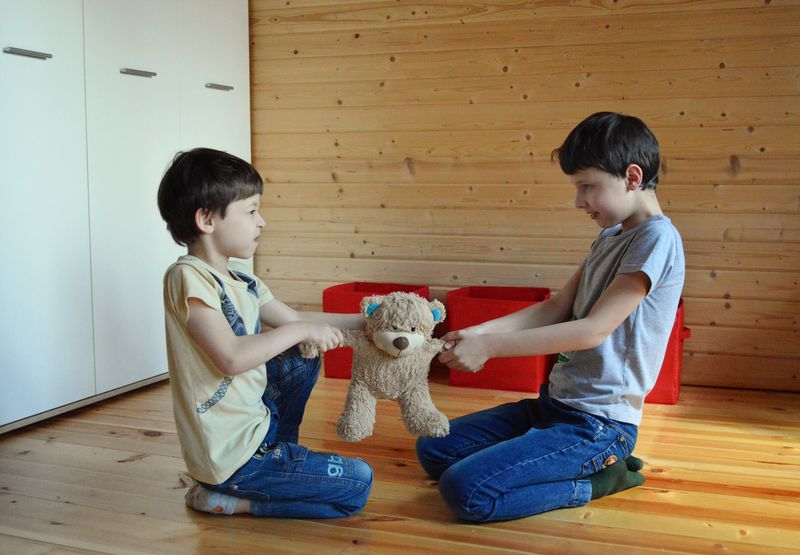
\includegraphics[width=\textwidth]{fig/siblings_toy.jpg}

      \vspace{0.3em}
      {\tiny\textcolor{lightgray}{Photo: Pexels (free license)}}
    \end{column}
  \end{columns}
  \pause
        \begin{insightbox}
        \centering Finite goods $\implies$ Rivalrous goods
      \end{insightbox}

\end{frame}

% ---------- Types of Goods ----------
\begin{frame}{Rivalrous goods}

  \begin{center}
  \begin{tikzpicture}[
    cell/.style={minimum width=4.8cm, minimum height=2cm, align=center,
                 font=\small, rounded corners=2pt},
    lbl/.style={font=\small\bfseries}
  ]
    % Column headers (black)
    \node[lbl, text=black] at (2.5,3.3) {Rivalrous};
    \node[lbl, text=black] at (7.5,3.3) {Non-rivalrous};

    % Grid lines
    \draw[DarkGray, thick] (0.3,-1.1) rectangle (9.7,2.9);
    \draw[DarkGray, thick] (5,-1.1) -- (5,2.9);
    \draw[DarkGray, thick] (0.3,0.9) -- (9.7,0.9);

    % Cells — examples only, no category labels
    \node[cell] at (2.65,2) {\textbullet~Store clothing\\\textbullet~Cars at a dealership};
    \node[cell] at (7.35,2) {\textbullet~Netflix movies\\\textbullet~Toll road};
    \node[cell] at (2.65,0) {\textbullet~Ocean fish\\\textbullet~Groundwater};
    \node[cell] at (7.35,0) {\textbullet~National defense\\\textbullet~Public parks};
  \end{tikzpicture}
  \end{center} \pause

  \begin{questionbox}
    Which items do you need to pay to use?
  \end{questionbox}

\end{frame}

% ---------- Types of Goods with Excludability ----------
\begin{frame}{Excludable Goods}

  \begin{center}
  \begin{tikzpicture}[
    cell/.style={minimum width=4.8cm, minimum height=2cm, align=center,
                 font=\small, rounded corners=2pt},
    lbl/.style={font=\small\bfseries}
  ]
    % Column headers (greyed out)
    \node[lbl, text=gray] at (2.5,3.3) {Rivalrous};
    \node[lbl, text=gray] at (7.5,3.3) {Non-rivalrous};

    % Row headers (black)
    \node[lbl, text=black, rotate=90, anchor=south] at (-0.6,1) {\normalsize Excludability};
    \node[lbl, text=black, rotate=90] at (-0.1,2) {High};
    \node[lbl, text=black, rotate=90] at (-0.1,0) {Low};

    % Grid lines
    \draw[DarkGray, thick] (0.3,-1.1) rectangle (9.7,2.9);
    \draw[DarkGray, thick] (5,-1.1) -- (5,2.9);
    \draw[DarkGray, thick] (0.3,0.9) -- (9.7,0.9);

    % Cells
    \node[cell] at (2.65,2) {\textbullet~Store clothing\\\textbullet~Cars at a dealership};
    \node[cell] at (7.35,2) {\textbullet~Netflix movies\\\textbullet~Toll road};
    \node[cell] at (2.65,0) {\textbullet~Ocean fish\\\textbullet~Groundwater};
    \node[cell] at (7.35,0) {\textbullet~National defense\\\textbullet~Public parks};
  \end{tikzpicture}
  \end{center} \pause

  \begin{definitionbox}[Excludable]
      A good is excludable when it's possible to prevent people who haven't paid from using it.
  \end{definitionbox}

\end{frame}

\begin{frame}{Excludable Goods}

  \begin{center}
  \begin{tikzpicture}[
    cell/.style={minimum width=4.8cm, minimum height=2cm, align=center,
                 font=\small, rounded corners=2pt},
    lbl/.style={font=\small\bfseries}
  ]
    % Column headers (greyed out)
    \node[lbl, text=gray] at (2.5,3.3) {Rivalrous};
    \node[lbl, text=gray] at (7.5,3.3) {Non-rivalrous};

    % Row headers (black)
    \node[lbl, text=black, rotate=90, anchor=south] at (-0.6,1) {\normalsize Excludability};
    \node[lbl, text=black, rotate=90] at (-0.1,2) {High};
    \node[lbl, text=black, rotate=90] at (-0.1,0) {Low};

    % Grid lines
    \draw[DarkGray, thick] (0.3,-1.1) rectangle (9.7,2.9);
    \draw[DarkGray, thick] (5,-1.1) -- (5,2.9);
    \draw[DarkGray, thick] (0.3,0.9) -- (9.7,0.9);

    % Cells
    \node[cell] at (2.65,2) {\textbullet~Store clothing\\\textbullet~Cars at a dealership};
    \node[cell] at (7.35,2) {\textbullet~Netflix movies\\\textbullet~Toll road};
    \node[cell] at (2.65,0) {\textbullet~Ocean fish\\\textbullet~Groundwater};
    \node[cell] at (7.35,0) {\textbullet~National defense\\\textbullet~Public parks};
  \end{tikzpicture}
  \end{center}

  \begin{questionbox}
    What type of good is the candy in Yale Policy 101?
  \end{questionbox}

\end{frame}

% ---------- Candy in the matrix ----------
\begin{frame}{Excludable Goods}

  \begin{center}
  \begin{tikzpicture}[
    cell/.style={minimum width=4.8cm, minimum height=2cm, align=center,
                 font=\small, rounded corners=2pt},
    lbl/.style={font=\small\bfseries}
  ]
    % Column headers (greyed out)
    \node[lbl, text=gray] at (2.5,3.3) {Rivalrous};
    \node[lbl, text=gray] at (7.5,3.3) {Non-rivalrous};

    % Row headers (black)
    \node[lbl, text=black, rotate=90, anchor=south] at (-0.6,1) {\normalsize Excludability};
    \node[lbl, text=black, rotate=90] at (-0.1,2) {High};
    \node[lbl, text=black, rotate=90] at (-0.1,0) {Low};

    % Grid lines
    \draw[DarkGray, thick] (0.3,-1.1) rectangle (9.7,2.9);
    \draw[DarkGray, thick] (5,-1.1) -- (5,2.9);
    \draw[DarkGray, thick] (0.3,0.9) -- (9.7,0.9);

    % Cells
    \node[cell] at (2.65,2) {\textbullet~Store clothing\\\textbullet~Cars at a dealership};
    \node[cell] at (7.35,2) {\textbullet~Netflix movies\\\textbullet~Toll road};
    \node[cell] at (2.65,0) {\textbullet~Ocean fish\\\textbullet~Groundwater\\[2pt]
      \textcolor{green}{\textbf{Yale candy}}};
    \node[cell] at (7.35,0) {\textbullet~National defense\\\textbullet~Public parks};
  \end{tikzpicture}
  \end{center}

\end{frame}

% ---------- Full labeled matrix ----------
\begin{frame}{Four Types of Goods}

  \begin{center}
  \begin{tikzpicture}[
    cell/.style={minimum width=4.8cm, minimum height=2cm, align=center,
                 font=\small, rounded corners=2pt},
    lbl/.style={font=\small\bfseries, text=black}
  ]
    % Column headers
    \node[lbl] at (2.5,3.3) {Rivalrous};
    \node[lbl] at (7.5,3.3) {Non-rivalrous};

    % Row headers
    \node[lbl, rotate=90, anchor=south] at (-0.6,1) {\normalsize Excludability};
    \node[lbl, rotate=90] at (-0.1,2) {High};
    \node[lbl, rotate=90] at (-0.1,0) {Low};

    % Grid lines
    \draw[DarkGray, thick] (0.3,-1.1) rectangle (9.7,2.9);
    \draw[DarkGray, thick] (5,-1.1) -- (5,2.9);
    \draw[DarkGray, thick] (0.3,0.9) -- (9.7,0.9);

    % Highlight common resources cell (fill within grid borders)
    \fill[orange!12] (0.3,-1.1) rectangle (5,0.9);

    % Cells with category labels and examples
    \node[cell] at (2.65,2) {\textbf{Private Goods}\\[2pt]
      {\scriptsize \textbullet~Store clothing \textbullet~Cars}};
    \node[cell] at (7.35,2) {\textbf{Club Goods}\\[2pt]
      {\scriptsize \textbullet~Netflix \textbullet~Toll road}};
    \node[cell] at (2.65,0) {\textbf{\textcolor{vermillion}{Common Resources}}\\[2pt]
      {\scriptsize \textbullet~Ocean fish \textbullet~Groundwater \textbullet~Yale candy}};
    \node[cell] at (7.35,0) {\textbf{Public Goods}\\[2pt]
      {\scriptsize \textbullet~National defense \textbullet~Public parks}};
  \end{tikzpicture}
  \end{center}

\end{frame}

% ---------- Tragedy of the Commons (1/2) ----------
\begin{frame}{Tragedy of the Commons}

  \begin{columns}[T]
    \begin{column}{0.55\textwidth}
      \begin{definitionbox}[Tragedy of the Commons]
        When individuals deplete a common resource. 
      \end{definitionbox}

      \vspace{0.3em}
      \textbf{Why it happens:}
      \begin{itemize}
        \item The good is \textbf{non-excludable} \& demand is infinite
        \item The good is \textbf{rivalrous} because supply is finite 
        \item The result is depletion 
      \end{itemize}
    \end{column}
    \begin{column}{0.42\textwidth}
      \centering
      {\small\textbf{Price = \$0 on a common resource}}

      \vspace{0.3em}
      \begin{tikzpicture}[scale=0.5]
        % Axes
        \draw[-{Stealth[length=4pt]}, thick] (0,0) -- (7.5,0)
          node[below, font=\small] {Quantity};
        \draw[-{Stealth[length=4pt]}, thick] (0,0) -- (0,5.5)
          node[above, font=\small] {Price};

        % Price line at zero
        \draw[vermillion, thick, dashed] (0,0.15) -- (7.2,0.15);
        \node[vermillion, font=\small\bfseries, anchor=east] at (-0.2,0.15) {\$0};

        % Demand curve
        \clip (-0.5,0) rectangle (7.5,5.3);
        \draw[blue, very thick, domain=0.25:7, smooth, samples=80]
          plot (\x, {3.2/(\x+0.15) + 0.2});

        % Label
        \node[blue, font=\small\bfseries] at (5.5,1.8) {Demand};
      \end{tikzpicture}

      \vspace{0.2em}
    \end{column}
  \end{columns} 
  \pause 
      \begin{questionbox}
        Why can't people self-regulate their behavior?
      \end{questionbox}

\end{frame}

% ---------- Self-Interest ----------
\begin{frame}{Self-Interest}

  \begin{columns}[T]
    \begin{column}{0.6\textwidth}
      \vspace{0.5em}
      \begin{quotebox}
        ``It is not from the benevolence of the butcher, the brewer, or the baker that we expect our dinner, but from their regard to their own interest.''

        \vspace{0.3em}
        \hfill --- Adam Smith, \textit{The Wealth of Nations} (1776)
      \end{quotebox}
    \end{column}
    \begin{column}{0.4\textwidth}
      \centering
      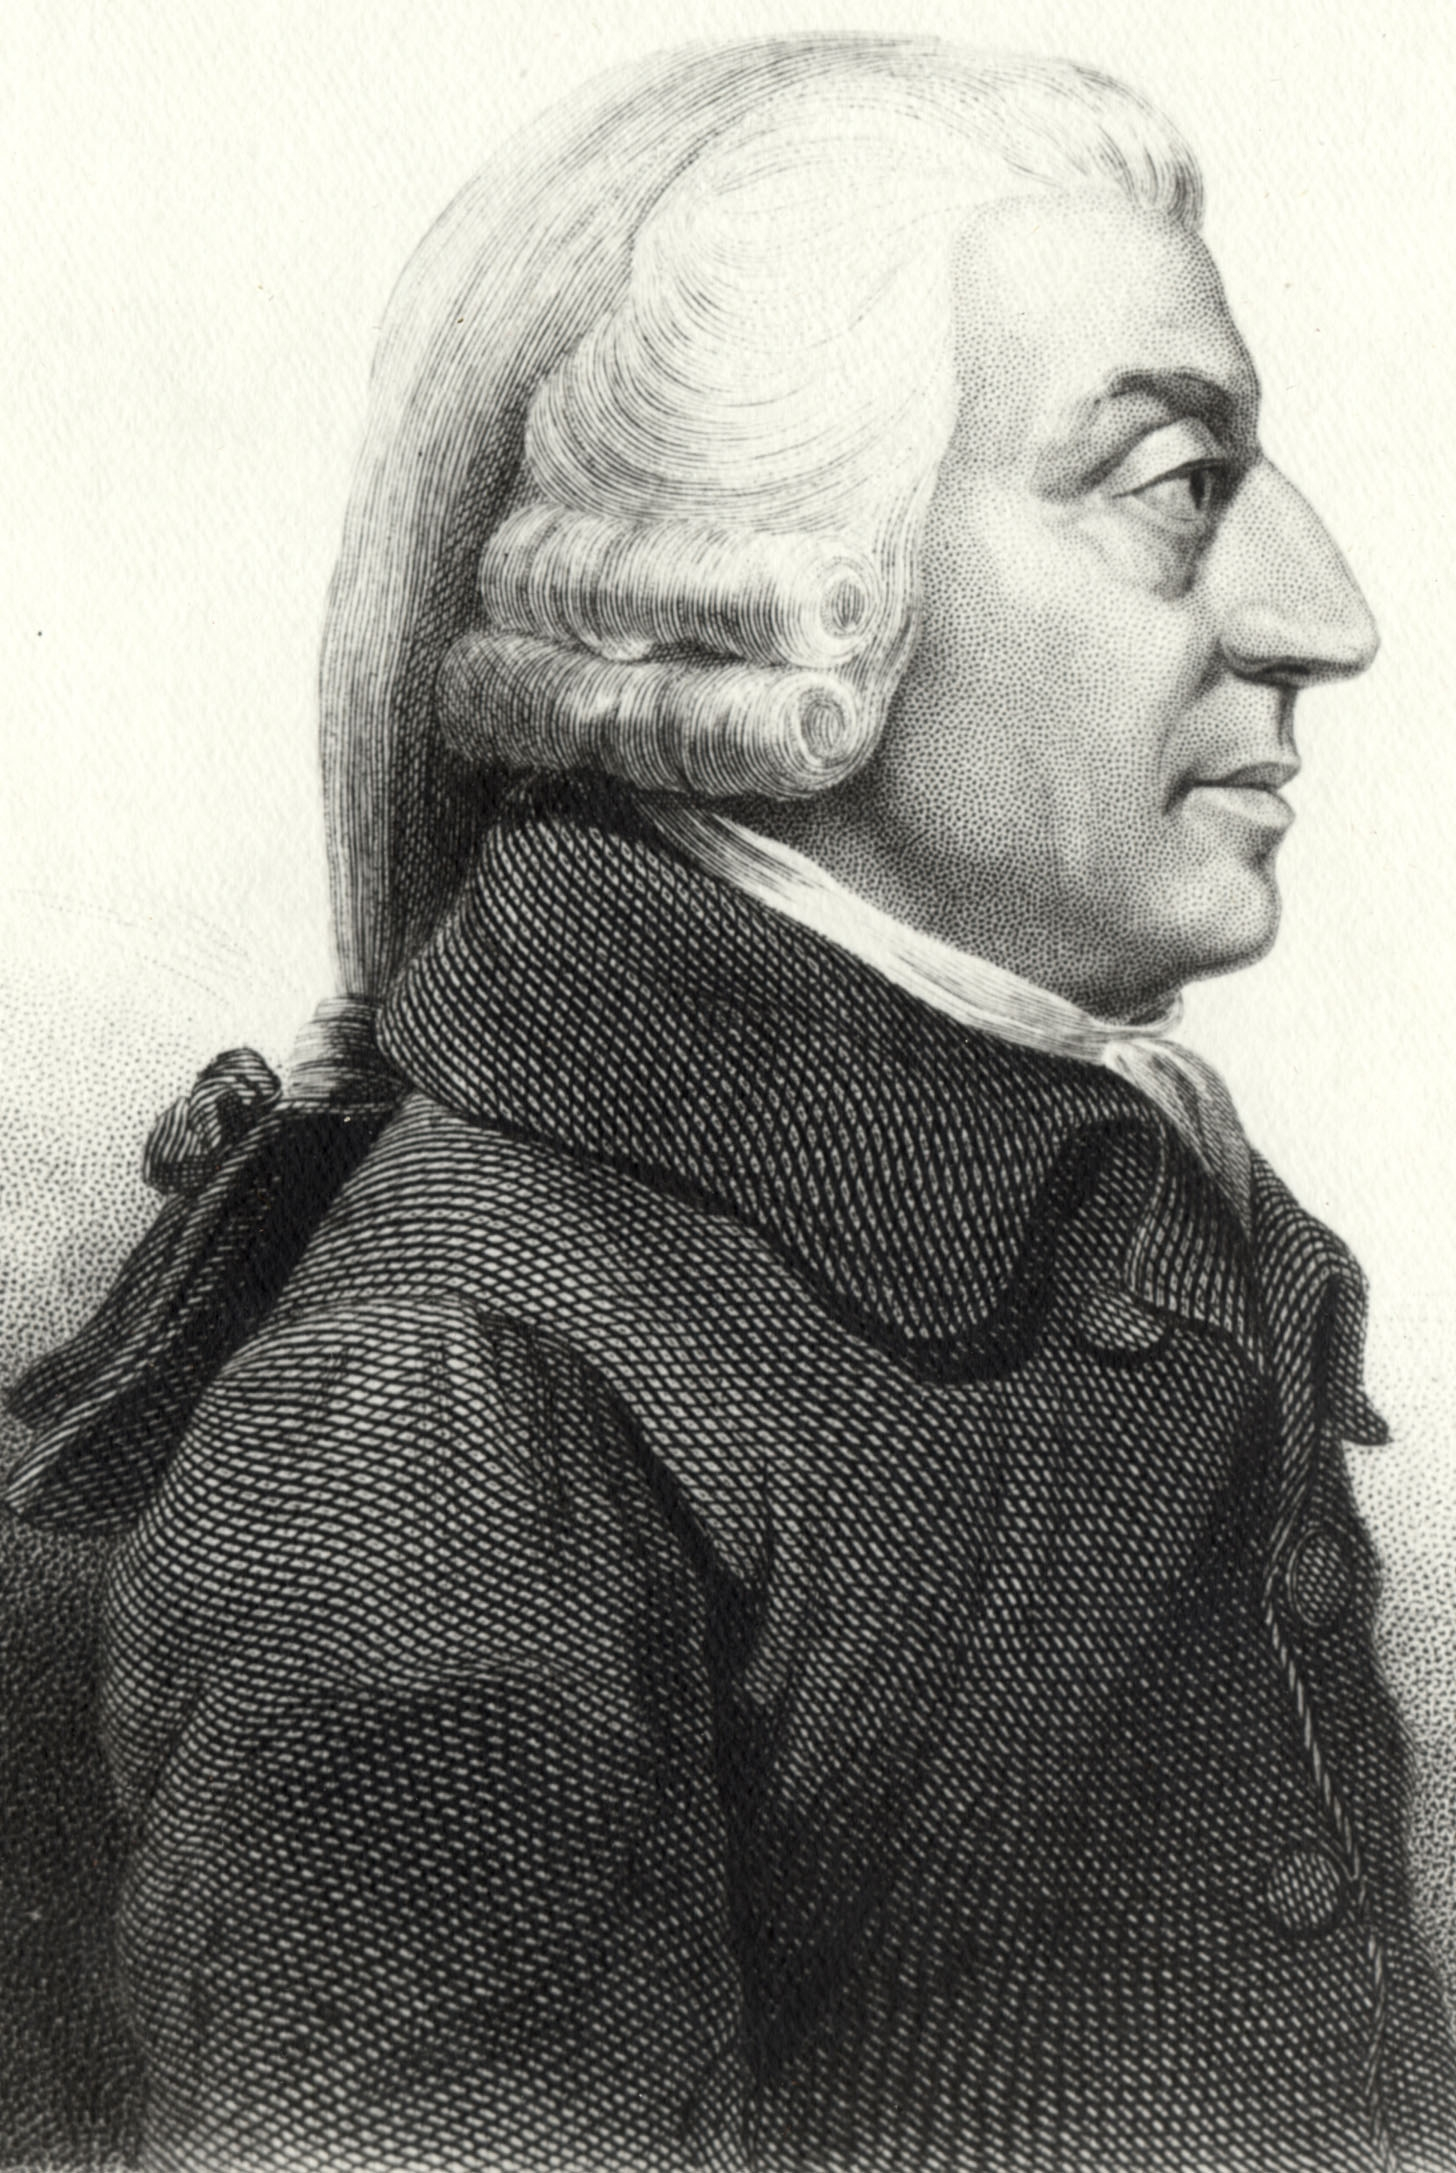
\includegraphics[width=\textwidth,height=3.5cm,keepaspectratio]{fig/adam_smith.jpg}

      \vspace{0.1em}
      {\scriptsize Adam Smith (1723--1790)\par}
    \end{column}
  \end{columns}

  \pause
  \vspace{0.3em}
  What is Adam Smith saying? 
  \begin{itemize}
    \item People act in their own interest to maximize their own happiness
    \item This is not greed --- it is \textbf{rational behavior}
    \item He argues that, overall, it's actually good for society that everyone acts this way! 
  \end{itemize}

  \vspace{0.3em}
  \begin{insightbox}
    Nobody is being ``bad,'' we are acting in our self-interest. This can have both good and bad outcomes.  
  \end{insightbox}
\end{frame}

% ---------- Negative Externalities ----------
\begin{frame}{Externalities}

  \begin{definitionbox}[Externality]
    An \textbf{externality} is a cost or benefit that affects someone \textbf{who is not directly involved} in a decision or transaction.
  \end{definitionbox}

  \vspace{0.5em}
  \begin{columns}[T]
    \begin{column}{0.48\textwidth}
      \textbf{\red{Negative} externality}
      \begin{itemize}
        \item Carbon emissions from driving $\rightarrow$ everyone faces climate change
      \end{itemize}
    \end{column}
    \begin{column}{0.48\textwidth}
      \textbf{\textcolor{green}{Positive} externality}
      \begin{itemize}
        \item A neighbor plants a beautiful garden $\rightarrow$ the whole street enjoys the view
      \end{itemize}
    \end{column}
  \end{columns}

  \vspace{0.5em} \pause
  \begin{questionbox}
    Which type of externality is the candy example?
  \end{questionbox}

\end{frame}

% ---------- Policy Solutions ----------
\begin{frame}{How Can We Fix the ``Tragedy of the Commons''?}

  \begin{definitionbox}[Tragedy of the Commons]
    When individuals deplete a common resource.
  \end{definitionbox}

  \vspace{0.3em}
  \begin{columns}[c]
    \begin{column}{0.48\textwidth}
      \centering
      {\small\textbf{Price = \$0 (Yale Policy 101)}}

      \vspace{0.3em}
      \begin{tikzpicture}[scale=0.55]
        % Axes
        \draw[-{Stealth[length=4pt]}, thick] (0,0) -- (7.5,0)
          node[below, font=\small] {Quantity};
        \draw[-{Stealth[length=4pt]}, thick] (0,0) -- (0,5.5)
          node[above, font=\small] {Price};

        % Price line
        \draw[vermillion, thick, dashed] (0,0.15) -- (7.2,0.15);
        \node[vermillion, font=\small\bfseries, anchor=east] at (-0.2,0.15) {\$0};

        % Demand curve
        \clip (-0.5,0) rectangle (7.5,5.3);
        \draw[blue, very thick, domain=0.25:7, smooth, samples=80]
          plot (\x, {3.2/(\x+0.15) + 0.2});

        % Label
        \node[blue, font=\small\bfseries] at (5.5,1.8) {Demand};
      \end{tikzpicture}
    \end{column}
    \pause
    \begin{column}{0.48\textwidth}
      \centering
      {\small\textbf{Price = \$5 (Yale Policy 102)}}

      \vspace{0.3em}
      \begin{tikzpicture}[scale=0.55]
        % Axes
        \draw[-{Stealth[length=4pt]}, thick] (0,0) -- (7.5,0)
          node[below, font=\small] {Quantity};
        \draw[-{Stealth[length=4pt]}, thick] (0,0) -- (0,5.5)
          node[above, font=\small] {Price};

        % Price line (higher up)
        \draw[vermillion, thick, dashed] (0,3.2) -- (7.2,3.2);
        \node[vermillion, font=\small\bfseries, anchor=east] at (-0.2,3.2) {\$5};

        % Demand curve
        \clip (-0.5,0) rectangle (7.5,5.3);
        \draw[blue, very thick, domain=0.25:7, smooth, samples=80]
          plot (\x, {3.2/(\x+0.15) + 0.2});

        % Label
        \node[blue, font=\small\bfseries] at (5.5,1.8) {Demand};

        % Vertical dotted line from intersection down to x-axis
        \draw[DarkGray, thick, dotted] (0.917,3.2) -- (0.917,0);
      \end{tikzpicture}
    \end{column}
  \end{columns}

  \pause
  \vspace{0.3em}
  \begin{insightbox}
    By raising the price, we reduce demand and prevent overuse.
    This is the logic behind taxes and fines.
  \end{insightbox}

\end{frame}

% ---------- Provocative Question ----------
% \begin{frame}{Something to Think About}

%   \vspace{2em}
%   \begin{questionbox}
%     Every time you ask ChatGPT a question, it uses electricity.
%     That electricity produces carbon emissions.

%     \vspace{0.5em}
%     \textbf{Should there be a price for polluting the air?}
%   \end{questionbox}

%   \vspace{1.5em}
%   \textit{We'll come back to this at the end of class.}

% \end{frame}


% ---------- Candy to Climate Change Comparison ----------
\begin{frame}{From Candy to Climate Change}

  \begin{columns}[T]
    \begin{column}{0.48\textwidth}
      \centering
      {\small\textbf{The Candy Problem}}

      \vspace{0.3em}
      \begin{tikzpicture}[
        nd/.style={rounded corners=3pt, draw=DarkGray, fill=softbg,
                   text width=3.8cm, minimum height=0.7cm,
                   align=center, font=\scriptsize},
        ar/.style={-{Stealth[length=3pt]}, thick, DarkGray}
      ]
        \node[nd, fill=vermillion!15, draw=vermillion] (obs) at (0,3.2)
          {\textbf{Candy runs out}};
        \node[nd] (why) at (0,2)
          {No price $\rightarrow$ everyone\\grabs as much as they want};
        \node[nd, fill=green!12, draw=green] (fix) at (0,0.8)
          {\textbf{Yale Policy 102}\\Charge \$5 per extra piece};
        \draw[ar] (obs) -- (why);
        \draw[ar] (why) -- (fix);
      \end{tikzpicture}
    \end{column} \pause
    \begin{column}{0.48\textwidth}
      \centering
      {\small\textbf{Climate Change}}

      \vspace{0.3em}
      \begin{tikzpicture}[
        nd/.style={rounded corners=3pt, draw=DarkGray, fill=softbg,
                   text width=3.8cm, minimum height=0.7cm,
                   align=center, font=\scriptsize},
        ar/.style={-{Stealth[length=3pt]}, thick, DarkGray}
      ]
        \node[nd, fill=vermillion!15, draw=vermillion] (obs) at (0,3.2)
          {\textbf{Planet warms up}};
        \node[nd] (why) at (0,2)
          {No price on CO\textsubscript{2} $\rightarrow$\\everyone pollutes freely};
        \node[nd, fill=green!12, draw=green] (fix) at (0,0.8)
          {\textbf{Carbon tax}\\Charge per ton of CO\textsubscript{2}};
        \draw[ar] (obs) -- (why);
        \draw[ar] (why) -- (fix);
      \end{tikzpicture}
    \end{column}
  \end{columns}

  \vspace{0.5em}
  \begin{insightbox}
    Same logic, bigger scale: the atmosphere is a common resource.
  \end{insightbox}

\end{frame}

% =============================================================================
\section{Carbon Tax Policy Discussion}
% =============================================================================

% ---------- Policy Discussion Header ----------
\begin{frame}{Policy Discussion}

  \vspace{2em}
  {\Huge\textbf{\textit{Should the U.S.\ put\\a price on carbon?}}}

\end{frame}

% ---------- Cause and Consequence ----------
\begin{frame}{The Cause and the Consequence}

  \begin{columns}[T]
    \begin{column}{0.48\textwidth}
      \centering
      {\small\textbf{Global CO\textsubscript{2} Emissions (Gt/yr)}}

      \vspace{0.2em}
      \begin{tikzpicture}[scale=0.42]
        % Axes
        \draw[-{Stealth[length=3pt]}, thick] (0,0) -- (12.5,0);
        \draw[-{Stealth[length=3pt]}, thick] (0,0) -- (0,6.5)
          node[above left, font=\tiny] {Gt/yr};

        % Y-axis labels
        \foreach \y/\lbl in {0/0, 1.5/10, 3/20, 4.5/30, 6/40} {
          \draw[DarkGray] (-0.15,\y) -- (0.15,\y);
          \node[font=\tiny, anchor=east] at (-0.2,\y) {\lbl};
        }

        % X-axis labels
        \foreach \x/\lbl in {0/1800, 4/1900, 6/1950, 8/1980, 10/2000, 12/2025} {
          \draw[DarkGray] (\x,-0.15) -- (\x,0.15);
          \node[font=\tiny, below] at (\x,-0.2) {\lbl};
        }

        % Emission curve
        \draw[blue, very thick] (0,0.01) -- (2,0.03) -- (4,0.3) -- (6,0.9)
          -- (8,3.0) -- (10,3.75) -- (12,5.7);

        % Data point labels
        \node[font=\tiny, blue, above] at (6,0.9) {6};
        \node[font=\tiny, blue, above] at (8,3.0) {20};
        \node[font=\tiny, blue, above left] at (12,5.7) {\textbf{38}};
      \end{tikzpicture}

      \vspace{0.2em}
      {\tiny Source: Global Carbon Project (2025).}
    \end{column}
    \begin{column}{0.48\textwidth}
      \centering
      {\small\textbf{Temperature Anomaly (\textdegree C vs.\ 1850--1900)}}

      \vspace{0.2em}
      \begin{tikzpicture}[scale=0.42]
        % Axes
        \draw[-{Stealth[length=3pt]}, thick] (0,-0.3) -- (12.5,-0.3);
        \draw[-{Stealth[length=3pt]}, thick] (0,-0.3) -- (0,7)
          node[above left, font=\tiny] {\textdegree C};

        % Y-axis labels (4 units = 1°C)
        \foreach \y/\lbl in {0/0, 2/{+0.5}, 4/{+1.0}, 6/{+1.5}} {
          \draw[DarkGray] (-0.15,\y) -- (0.15,\y);
          \node[font=\tiny, anchor=east] at (-0.2,\y) {\lbl};
        }

        % Zero line
        \draw[DarkGray, dashed, thin] (0,0) -- (12,0);

        % X-axis labels
        \foreach \x/\lbl in {0/1880, 4/1920, 8/1960, 10/1980, 12/2025} {
          \draw[DarkGray] (\x,-0.45) -- (\x,-0.15);
          \node[font=\tiny, below] at (\x,-0.45) {\lbl};
        }

        % 1.5°C target line
        \draw[orange, thick, dashed] (0,6) -- (12,6);
        \node[orange, font=\tiny, anchor=west] at (12.2,6) {1.5\textdegree C};

        % Temperature curve
        \fill[vermillion!15] (0,-0.4) -- (2,0) -- (4,-0.2) -- (6,0.6)
          -- (8,0.2) -- (10,1.2) -- (11,2.6) -- (12,6.0)
          -- (12,-0.3) -- (0,-0.3) -- cycle;

        \draw[vermillion, very thick] (0,-0.4) -- (2,0) -- (4,-0.2) -- (6,0.6)
          -- (8,0.2) -- (10,1.2) -- (11,2.6) -- (12,6.0);

        % Key label
        \node[font=\tiny, vermillion, above left] at (12,6.0) {\textbf{+1.5\textdegree C}};
      \end{tikzpicture}

      \vspace{0.2em}
      {\tiny Source: NASA GISS; Copernicus.}
    \end{column}
  \end{columns}

  \vspace{0.3em}
  \begin{insightbox}
    Most emissions have occurred in the last 70 years.
    The Earth is now 1.5\textdegree C warmer --- right at the Paris Agreement target.
  \end{insightbox}

\end{frame}

% ---------- Who Emits in the US ----------
\begin{frame}{Who Emits in the U.S.?}

  \textbf{U.S.\ Greenhouse Gas Emissions by Sector (2022)}
  \centering
  \vspace{0.3em}
  {\small
  \begin{tabular}{@{} l c p{3.2cm} p{3.2cm} @{}}
    \toprule
    \textbf{Sector} & \textbf{\%} & \textcolor{skyblue}{\textbf{Households}} & \textcolor{orange}{\textbf{Firms}} \\
    \midrule
    Transportation & 28\% &
      Cars, personal trucks &
      Freight, airlines, shipping \\[0.4em]
    Electric Power & 25\% &
      Home electricity use &
      Factory \& office electricity \\[0.4em]
    Industry & 23\% &
      --- &
      Manufacturing, refining, chemicals \\[0.4em]
    Comm.\ \& Residential & 13\% &
      Home heating, refrigerants &
      Office \& retail heating \\[0.4em]
    Agriculture & 10\% &
      --- &
      Livestock, crops, fertilizer \\
    \bottomrule
  \end{tabular}
  }

  % \vspace{0.5em}
  % \begin{insightbox}
  %   Every sector has a mix of household and firm emissions.
  %   A carbon tax would affect \textbf{both} --- the question is \textbf{who pays more}.
  % \end{insightbox}

  \vspace{0.2em}
  {\tiny Source: U.S.\ EPA, \textit{Inventory of U.S.\ Greenhouse Gas Emissions and Sinks: 1990--2022}.}

\end{frame}

% ---------- Policy Proposal: Carbon Tax ----------
\begin{frame}{A Policy Proposal: Tax Carbon Emissions}

  \begin{definitionbox}[Carbon Tax]
    A fixed price charged for every \textbf{ton of CO\textsubscript{2}} emitted.
    The polluter pays for the damage their emissions cause.
  \end{definitionbox}

  \vspace{0.5em}
  \begin{columns}[T]
    \begin{column}{0.48\textwidth}
      \textbf{How it works:}
      \begin{itemize}
        \item Government sets a price, e.g.\ \textbf{\$50 per ton} of CO\textsubscript{2}
        \item Firms and households pay when they emit

      \end{itemize}
    \end{column}
  \end{columns}

\end{frame}

% ---------- What Does This Mean at the Gas Pump ----------
\begin{frame}{What Does \$50 per Ton of CO\textsubscript{2} Mean?}

  \begin{columns}[T]
    \begin{column}{0.40\textwidth}
      \begin{answerbox}
        \centering
        Gas price: \$3.50 $\rightarrow$ \textbf{\$3.94}\\[0.3em]
        {\small An increase of about \textbf{13\%}}
      \end{answerbox}

      \vspace{0.3em}
      {\tiny Source: EPA, ``Greenhouse Gases Equivalencies Calculator.''\\
       Average U.S.\ gas price as of 2025.}
    \end{column}
    \pause
    \begin{column}{0.56\textwidth}
      \centering
      {\small\textbf{Who is affected?}}

      \vspace{0.3em}
      \begin{tikzpicture}[
        grp/.style={rounded corners=3pt, minimum width=2.2cm,
                    minimum height=1.4cm, align=center, font=\scriptsize},
      ]
        % Firms — factory icon
        \node[grp, draw=blue, fill=blue!8] (firms) at (0,1.5) {};
        \fill[blue!60] (-0.4,1.65) rectangle (0.2,1.95);
        \fill[blue!60] (0.25,1.75) rectangle (0.4,1.95);
        \node[font=\scriptsize\bfseries] at (0,1.25) {Firms};

        % Households — house icon
        \node[grp, draw=orange, fill=orange!8] (hh) at (2.8,1.5) {};
        \fill[orange!60] (2.5,1.55) rectangle (3.1,1.8);
        \fill[orange!60] (2.5,1.8) -- (2.8,2.0) -- (3.1,1.8) -- cycle;
        \node[font=\scriptsize\bfseries] at (2.8,1.25) {Households};

        % High income — large stick figure
        \node[grp, draw=green, fill=green!8] (rich) at (0,0) {};
        \draw[green!70!black, thick] (0,0.55) circle (0.12);
        \draw[green!70!black, thick] (0,0.43) -- (0,0.15);
        \draw[green!70!black, thick] (-0.15,0.35) -- (0.15,0.35);
        \draw[green!70!black, thick] (0,0.15) -- (-0.12,0.0) (0,0.15) -- (0.12,0.0);
        \node[font=\scriptsize\bfseries, below] at (0,-0.15) {High income};

        % Low income — small stick figure
        \node[grp, draw=vermillion, fill=vermillion!8] (poor) at (2.8,0) {};
        \draw[vermillion, thick] (2.8,0.4) circle (0.1);
        \draw[vermillion, thick] (2.8,0.3) -- (2.8,0.1);
        \draw[vermillion, thick] (2.68,0.22) -- (2.92,0.22);
        \draw[vermillion, thick] (2.8,0.1) -- (2.7,0.0) (2.8,0.1) -- (2.9,0.0);
        \node[font=\scriptsize\bfseries, below] at (2.8,-0.15) {Low income};
      \end{tikzpicture}


    \end{column}
  \end{columns}

\end{frame}

% ---------- Government Revenue ----------
\begin{frame}{What Should the Government Do with the Revenue?}

  A carbon tax generates \textbf{billions of dollars} in revenue every year.
  The government has three main options:

  \vspace{0.5em}
  \begin{center}
  \begin{tikzpicture}[
    nd/.style={rounded corners=3pt, draw=DarkGray, fill=softbg,
               text width=3.2cm, minimum height=0.8cm,
               align=center, font=\small},
    ar/.style={-{Stealth[length=4pt]}, thick, DarkGray}
  ]
    % Revenue source
    \node[nd, fill=blue!12, draw=blue, text width=4cm] (rev) at (0,2.5)
      {\textbf{Carbon Tax Revenue}};

    % Three options
    \node[nd, fill=orange!12, draw=orange] (opt1) at (-4,0.5)
      {\textbf{Return to households}\\[2pt] as rebate checks};
    \node[nd, fill=skyblue!12, draw=skyblue] (opt2) at (0,0.5)
      {\textbf{Invest}\\[2pt] in firms to reduce CO\textsubscript{2}};
    \node[nd, fill=green!12, draw=green] (opt3) at (4,0.5)
      {\textbf{Cut other taxes}\\[2pt] e.g.\ income tax};

    \draw[ar] (rev) -- (opt1);
    \draw[ar] (rev) -- (opt2);
    \draw[ar] (rev) -- (opt3);
  \end{tikzpicture}
  \end{center}

\end{frame}

% ---------- Canada's Real-World Example ----------
\begin{frame}{Real-World Example: Canada}

  \begin{columns}[c]
    \begin{column}{0.48\textwidth}
      \centering
      \begin{tikzpicture}[scale=0.75]
        % Newspaper frame
        \draw[black, thick] (0,0) rectangle (5,6.5);
        % Masthead
        \fill[vermillion!15] (0,5.5) rectangle (5,6.5);
        \node[font=\large\bfseries\scshape] at (2.5,6.2) {The Globe and Mail};
        \draw[black, thin] (0.3,5.7) -- (4.7,5.7);
        \node[font=\tiny] at (2.5,5.85) {Toronto, ON \quad 2024};
        % Headline
        \node[text width=4.2cm, align=center, font=\small\bfseries]
          at (2.5,4.8) {CANADA PRICES CARBON:\\CA\$80 per Ton of CO\textsubscript{2}};
        % Sub-headline
        \node[text width=4.2cm, align=center, font=\scriptsize]
          at (2.5,3.9) {90\% of revenue returned\\directly to households};
        % Divider
        \draw[black, thin] (0.3,3.4) -- (4.7,3.4);
        % Fake article body (gray lines)
        \foreach \y in {3.1,2.85,2.6,2.35,2.1,1.85,1.6,1.35,1.1,0.85,0.6}
          \fill[gray!40] (0.4,\y) rectangle (4.6,\y+0.12);
      \end{tikzpicture}
    \end{column}
    \begin{column}{0.48\textwidth}
      \textbf{What happened:}
      \begin{itemize}
        \item Canada introduced a carbon tax of \textbf{CA\$80/ton} in 2024
        \item \textbf{90\%} of revenue is returned to households via quarterly rebate checks
        \item \textbf{8 out of 10 households get back more} than they pay in higher prices
      \end{itemize}

      \vspace{0.3em}
      {\tiny Source: Canada Parliamentary Budget Officer (2024).}
    \end{column}
  \end{columns}

\end{frame}

% ---------- Stakeholder Hearing ----------
\begin{frame}{Policy Debate}

  \begin{columns}[c]
    \begin{column}{0.48\textwidth}
      \begin{questionbox}
        \textbf{Economic analysis:} Should the U.S.\ put a price on carbon?
      \end{questionbox}

      \vspace{0.5em}
      Three stakeholder groups will analyze the question:
      \begin{itemize}
        \item Households
        \item Firms
        \item Government
      \end{itemize}

    \end{column}
    \begin{column}{0.48\textwidth}
      \textbf{Your Task:} For your assigned group, answer:
      \vspace{0.3em}

      \begin{enumerate}
        \item What are the \textcolor{green}{benefits} of a carbon tax for your group?
        \vspace{0.3em}
        \item What are the \textcolor{vermillion}{costs} of a carbon tax for your group?
        \vspace{0.3em}
        \item What is your \textbf{policy recommendation}? Choose one of the following:
        \begin{enumerate}
          \item No tax
          \item Tax + rebate to households 
          \item Tax + green investment 
          \item Other (formulate your own policy!) 
        \end{enumerate}
      \end{enumerate}

    \end{column}
  \end{columns}

\end{frame}

% ---------- Stakeholder Analysis: Households ----------
\begin{frame}{Stakeholder Analysis: Households}

  \begin{columns}[T]
    \begin{column}{0.48\textwidth}
      \textbf{\textcolor{green!60!black}{Benefits}}
      \begin{itemize}\small
        \item Cleaner air $\rightarrow$ fewer health problems (asthma, heart disease)
        \item Rebate checks could exceed what most families pay in higher prices
        \item Drives innovation in affordable clean energy
        \item Protects future generations from climate damage
      \end{itemize}
    \end{column}
    \begin{column}{0.48\textwidth}
      \textbf{\textcolor{vermillion}{Costs}}
      \begin{itemize}\small
        \item Higher gas, electricity, and heating bills
        \item Poor households spend a larger share of income on energy
        \item Rural families with no transit alternatives are hit hardest
        \item Higher prices on everyday goods (food, shipping)
      \end{itemize}
    \end{column}
  \end{columns}

\end{frame}

% ---------- Stakeholder Analysis: Firms ----------
\begin{frame}{Stakeholder Analysis: Firms}

  \begin{columns}[T]
    \begin{column}{0.48\textwidth}
      \textbf{\textcolor{green!60!black}{Benefits}}
      \begin{itemize}\small
        \item Clear price signal helps long-term planning
        \item Early movers gain competitive advantage in clean technology
        \item Level playing field if all firms face the same carbon price
        \item New markets for low-carbon products and services
      \end{itemize}
    \end{column}
    \begin{column}{0.48\textwidth}
      \textbf{\textcolor{vermillion}{Costs}}
      \begin{itemize}\small
        \item Higher production costs (energy, raw materials)
        \item Disadvantage vs.\ foreign competitors without a carbon tax
        \item Energy-intensive industries may relocate abroad (``carbon leakage'')
        \item Short-run job losses in fossil fuel sectors (coal, oil, gas)
      \end{itemize}
    \end{column}
  \end{columns}

\end{frame}

% ---------- Stakeholder Analysis: Government ----------
\begin{frame}{Stakeholder Analysis: Government}

  \begin{columns}[T]
    \begin{column}{0.48\textwidth}
      \textbf{\textcolor{green!60!black}{Benefits}}
      \begin{itemize}\small
        \item New revenue stream (\$250B/year at \$50/ton)
        \item Meets international climate commitments (Paris Agreement)
        \item Reduces future costs of climate disasters (floods, wildfires)
        \item Market-based approach --- less bureaucracy than regulations
      \end{itemize}
    \end{column}
    \begin{column}{0.48\textwidth}
      \textbf{\textcolor{vermillion}{Costs}}
      \begin{itemize}\small
        \item Political backlash --- voters dislike higher energy prices
        \item Administrative cost of implementing and enforcing the tax
        \item If the U.S.\ acts alone, global emissions may not fall much
        \item Revenue spent on rebates cannot fund other priorities
      \end{itemize}
    \end{column}
  \end{columns}

\end{frame}

% =============================================================================
\section{Recap}
% =============================================================================

\begin{frame}{Today's Key Takeaways}

  \begin{enumerate}
    \item The \textbf{Tragedy of the Commons} arises when goods are \textbf{common resources}:
    \begin{itemize}
      \item \textbf{Rivalrous} 
      \item \textbf{Non-excludable}
    \end{itemize}
    \vspace{0.5em}
    \item People demand too much and \textbf{deplete} the resource.
    This imposes a \textbf{negative externality} on others: they lose the opportunity to consume.
    \vspace{0.5em}

    \item This problem can be mitigated with a \textbf{price system},
    which changes incentives and generates revenue.
    \vspace{0.5em}

    \item We applied this logic to \textbf{climate change}
    \vspace{0.5em}

    \item But there are \textbf{always costs} to such policies! Different stakeholders
    (households, firms, government) are affected differently.
  \end{enumerate}

\end{frame}


\end{document}
